\documentclass[11pt]{article}
\usepackage{acl_style}
\usepackage{enumitem}
\usepackage{float}
\usepackage{caption}
\usepackage{subcaption}
\usepackage{tabularx}
\usepackage{array}
\usepackage{multirow}
\usepackage{subcaption}
\usepackage{tikz}
\usetikzlibrary{shapes.geometric, arrows.meta, positioning, calc, fit}
% --- CUSTOM COMMANDS & COLORS ---
\newcommand{\subtitle}[1]{{\scriptsize #1}} % FIXED: Defined missing subtitle command
\newcommand{\sub}[1]{{\footnotesize #1}} % Defines \sub as small text


% Define custom colors (can be placed here or inside the document)
\definecolor{boxblue}{RGB}{235, 245, 255}
\definecolor{borderblue}{RGB}{100, 149, 237}
\definecolor{boxgreen}{RGB}{232, 245, 233}
\definecolor{bordergreen}{RGB}{76, 175, 80}
\definecolor{boxpurple}{RGB}{243, 229, 245}
\definecolor{borderpurple}{RGB}{156, 39, 176}
\definecolor{boxorange}{RGB}{255, 243, 224}
\definecolor{borderorange}{RGB}{255, 152, 0}
\definecolor{boxgray}{RGB}{238, 238, 238}
\definecolor{bordergray}{RGB}{158, 158, 158}

\hypersetup{colorlinks=true,linkcolor=blue!60!black,citecolor=blue!60!black,urlcolor=blue!60!black}

\setlist{nosep,leftmargin=1.2em}

\title{RepoQA: A Retrieval-Augmented Question Answering System\\for Understanding GitHub Repositories}

\author{
  \textbf{Sushmi Shrestha} \\
  Faculty of Advanced Science and Technology \\
  Asian Institute of Technology\\
  \texttt{st126526@ait.asia}
}

\date{}

\begin{document}
\maketitle

% ============================================================
% ABSTRACT
% ============================================================
\begin{abstract}
Developers spend the majority of their time reading and understanding code, yet current AI coding assistants primarily focus on code generation and completion. When developers encounter an unfamiliar repository, they face questions about architecture (``How does authentication work here?''), code logic (``What does this middleware do?''), and deployment (``How is this service configured?'') that existing tools cannot reliably answer. This \textbf{RepoQA}, a retrieval-augmented question answering system that helps developers understand GitHub repositories through natural language interaction. The approach introduces three key innovations: (1)~a hierarchical summarization pipeline that generates project-, directory-, and file-level descriptions to enable multi-level understanding; (2)~a hybrid retrieval engine combining semantic search, BM25 keyword matching, and dependency-graph traversal with question-type-aware routing; and (3)~structured explanation prompts that produce grounded, citation-rich answers. The evaluation of RepoQA on the CoReQA benchmark (1,563 QA pairs from 176 repositories across four programming languages) using the LLM-as-a-judge framework. The experiments aim to demonstrate that hierarchical hybrid retrieval significantly outperforms the BM25 baseline reported in prior work (accuracy: 6.91/10, completeness: 6.34/10) and investigate the contribution of each architectural component through comprehensive ablation studies. This work addresses the critical gap between code generation tools and developer comprehension needs, advancing the state of repository-level code understanding.
\end{abstract}

% ============================================================
% 1. INTRODUCTION (Wobbrock 5-part structure)
% ============================================================
\section{Introduction}

% Part 1: Problem / Motivation
Software development is fundamentally a comprehensive activity. Studies consistently report that developers spend 58--70\% of their time reading and understanding existing code rather than writing new code \citep{xia2018measuring}. When onboarding to an unfamiliar repository, developers face a barrage of questions: \textit{How is this project structured? What does this function do? Why was this design pattern chosen? How do I deploy this service locally?} These questions span multiple levels of abstraction---from high-level architecture down to individual function logic---and frequently require tracing dependencies across multiple files.

% Part 2: Gap in existing work
Despite rapid advances in AI-powered coding tools, the current landscape exhibits a fundamental mismatch. Tools such as GitHub Copilot \citep{chen2021evaluating}, Cursor excel at code completion and generation but are not designed for code understanding and explanation. On the research side, most benchmarks target code generation \citep{chen2021evaluating, austin2021program} or bug fixing \citep{jimenez2024swebench}, with limited attention to question answering. Recent work by \citet{chen2025coreqa} demonstrates this gap starkly: even GPT-4o with BM25 retrieval scores only 6.91/10 on accuracy for repository-level QA, and completeness scores languish at 6.34/10. The authors attribute this to BM25's inability to capture semantic relationships in code, where terms exhibit minimal variation and keyword matching misses crucial context.

% Part 3: The approach
To address this gap, the \textbf{RepoQA}, a retrieval-augmented question answering system designed specifically for repository-level code comprehension. RepoQA introduces three innovations. First, develop a \textit{hierarchical summarization pipeline} that generates project-, directory-, and file-level summaries, enabling the system to answer questions at multiple levels of abstraction (following \citealp{tufek2025hierarchical}). Second, design a \textit{hybrid retrieval engine} that fuses semantic search, BM25, and dependency-graph traversal, with a question-type router that selects the appropriate retrieval strategy based on whether the question targets architecture, logic, or deployment. Third, employ \textit{structured explanation prompts} that organize context top-down (project summary $\rightarrow$ directory summary $\rightarrow$ code chunks) and require the LLM to cite specific files and line numbers, directly optimizing for the accuracy and completeness dimensions identified as challenging by \citet{chen2025coreqa}.

% Part 4: Contributions
This paper makes the following contributions:
\begin{enumerate}
    \item Formalize the task of repository-level question answering with a taxonomy of developer questions (architecture, logic, deployment) and propose a multi-level retrieval strategy tailored to each question type.
    \item Design a complete RAG pipeline with hierarchical summarization, hybrid retrieval, and structured prompt generation for code explanation.
    \item Provide a comprehensive evaluation plan using the CoReQA benchmark with LLM-as-a-judge evaluation across four quality dimensions, including ablation studies isolating the contribution of each component.
\end{enumerate}

% Part 5: Research questions
This work is guided by the following three research questions:

\noindent\textbf{RQ1:} Does hierarchical hybrid retrieval (semantic + BM25 + structural) significantly improve answer quality over BM25-only retrieval for repository-level code QA?

\noindent\textbf{RQ2:} How does question-type-aware routing (architecture vs.\ logic vs.\ deployment) affect retrieval precision and answer completeness compared to a uniform retrieval strategy?

\noindent\textbf{RQ3:} What is the individual contribution of each system component (hierarchical summaries, hybrid fusion, query expansion, structured prompts) to overall QA performance?

% Expected results
The hypotheses are -- (1) hybrid retrieval will outperform BM25 by at least 0.5 points on accuracy and completeness (CoReQA scale), driven by semantic search capturing conceptual relevance that BM25 misses; (2) question-type routing will most benefit architecture questions, which require broad context, while logic questions will benefit most from function-level retrieval; and (3) hierarchical summaries will have the largest individual impact on completeness, as they provide the multi-level context needed to address all aspects of a question.

% ============================================================
% 2. RELATED WORK
% ============================================================
\section{Related Work}

\subsection{Code Question Answering}

Early code QA research focuses on snippet-level understanding. \citet{liu2021codeqa} introduce CodeQA, generating QA pairs from code comments at the function level, while CS1QA \citep{lee2022cs1qa} targets introductory programming education. These benchmarks are limited to isolated code fragments and do not address the cross-file reasoning required in real-world repositories.

Recent work has shifted toward repository-level QA. \citet{chen2025coreqa} introduce CoReQA, constructing 1,563 QA pairs from GitHub issues and comments across 176 repositories in four languages. Their evaluation reveals that even GPT-4o scores below 7/10 on accuracy, with BM25 providing negligible improvement. \citet{peng2025sweqa} propose SWE-QA, specifically targeting module-level architectural comprehension---understanding how modules interact, their architectural roles, and semantic contracts between them. \citet{strich2024improving} present a self-alignment pipeline for repository code QA at ACL~2024, using RAG over the Spyder IDE codebase. CodeRepoQA \citep{coderepoqa2024} offers a complementary multi-turn benchmark derived from repository discussions.

\textbf{Gap:} While these benchmarks define the problem, none propose a comprehensive retrieval solution. CoReQA identifies BM25's inadequacy but does not explore alternatives. SWE-QA introduces an agent-based approach but lacks ablation analysis. The work directly addresses the retrieval gap by proposing and evaluating a hierarchical hybrid pipeline.

\subsection{Retrieval-Augmented Generation for Code}

RAG has become the dominant paradigm for augmenting LLMs with external knowledge \citep{gao2024rag}. In the code domain, RepoCoder \citep{zhang2023repocoder} introduces an iterative retrieval-generation loop for code completion, while DraCo \citep{cheng2024draco} uses dataflow-guided retrieval. CAST \citep{cast2025} demonstrates that AST-aware chunking outperforms fixed-size chunking for code RAG. CodeRAG-Bench \citep{wang2025coderag} provides a systematic evaluation of 10 retrievers and 10 LMs on code generation tasks.

\textbf{Gap:} These approaches optimize retrieval for code \textit{completion}, not code \textit{understanding}. The retrieved context for completion (next token prediction) differs fundamentally from what is needed for explanation (architectural context, design rationale, cross-file dependencies). The work adapts RAG for the explanation task through hierarchical summarization and question-type routing.

\subsection{Repository-Level Code Understanding}

\citet{tufek2025hierarchical} propose hierarchical summarization that constructs project-, directory-, and file-level summaries for bug localization, achieving state-of-the-art results by guiding LLMs through a top-down search. CodePlan \citep{bairi2024codeplan} frames repository-level tasks as planning problems but targets code editing, not comprehension. Gistify \citep{gistify2025} evaluates codebase-level understanding through execution-based metrics but does not propose a retrieval method.

\textbf{Gap:} Hierarchical summarization has been applied to code search and bug localization, but not to developer-facing QA. Adapt and extend this approach specifically for the question-answering setting, combining it with hybrid retrieval and structured explanation prompts.

% ============================================================
% 3. METHODOLOGY
% ============================================================
\section{Methodology}

Figure~\ref{fig:architecture} presents the overall architecture of RepoQA, which consists of four main components: (1)~repository ingestion and hierarchical summarization, (2)~hybrid retrieval with question-type routing, (3)~structured prompt generation, and (4)~answer generation with grounding verification.

\begin{figure*}[ht]
\centering
\resizebox{\textwidth}{!}{
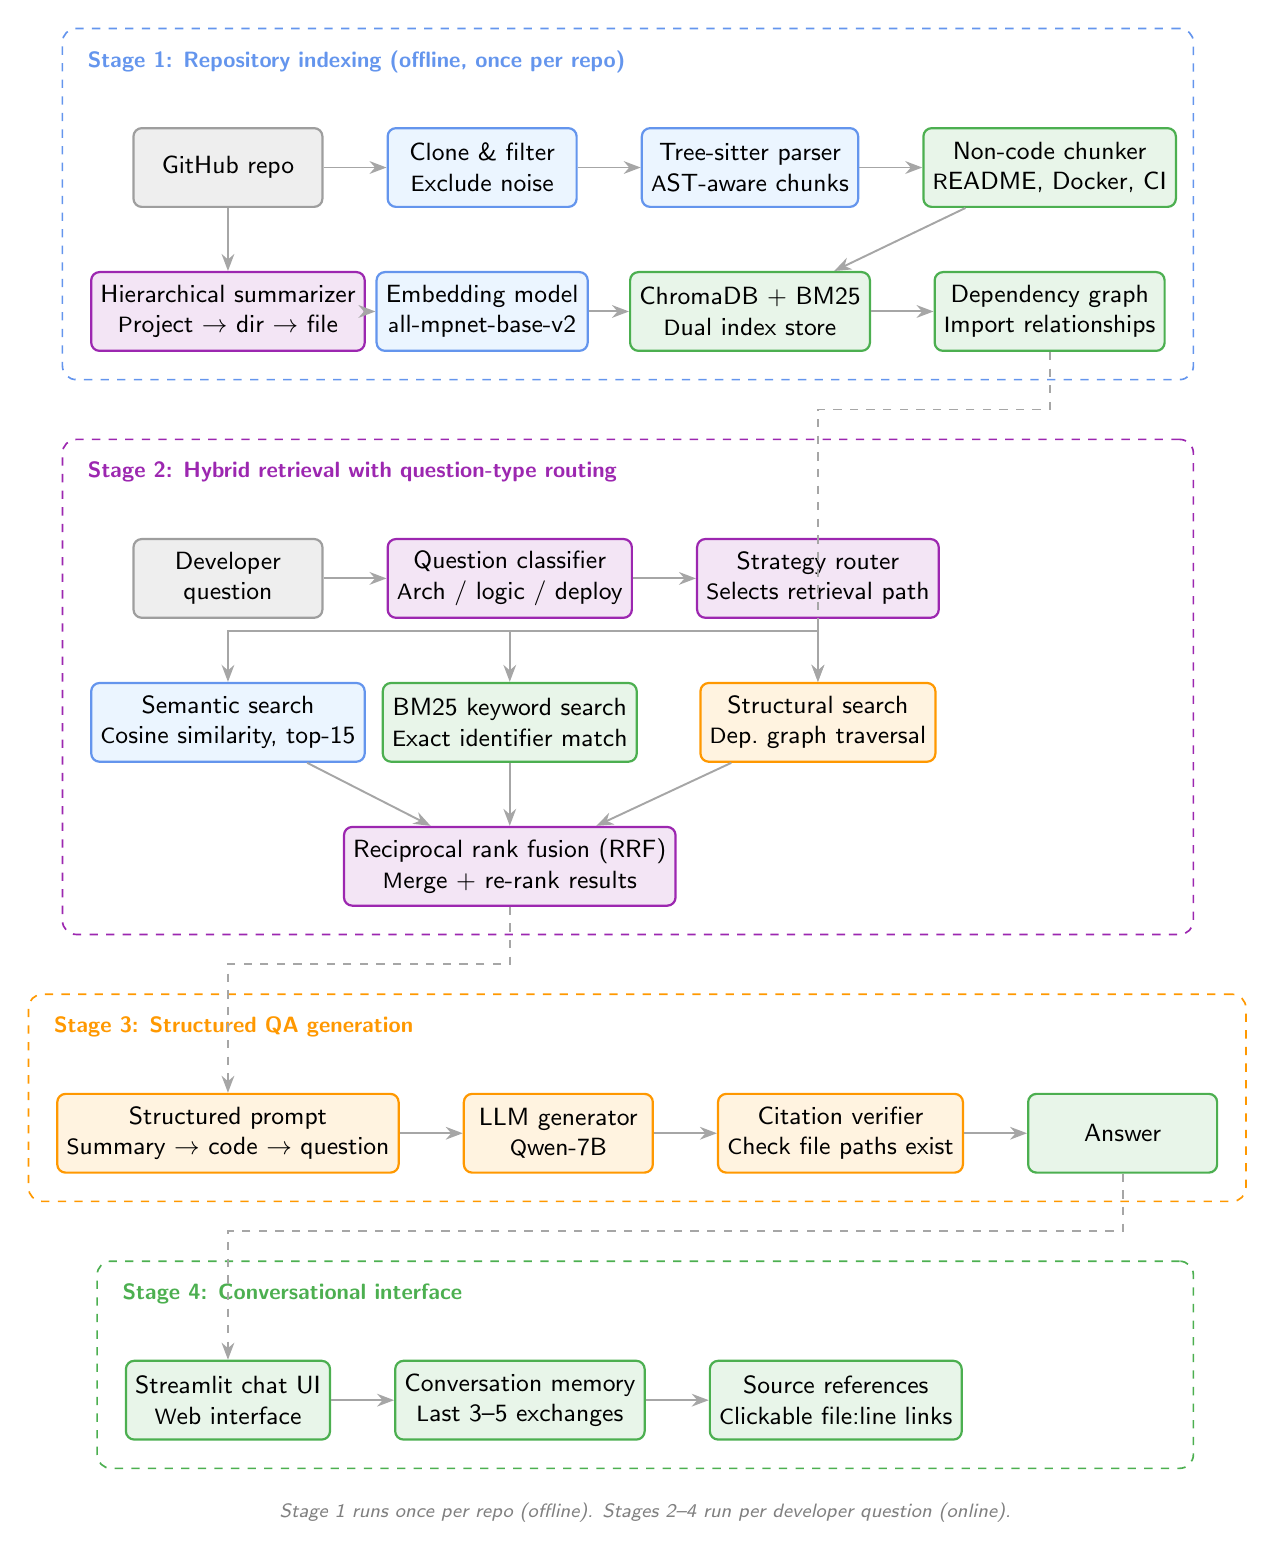
\begin{tikzpicture}[
    font=\sffamily\small,
    node distance=0.8cm and 0.8cm,
    base/.style={rectangle, rounded corners=3pt, draw, align=center,
                 minimum height=1cm, minimum width=2.4cm, line width=0.8pt},
    sub/.style={font=\sffamily\scriptsize},
    graybox/.style={base, fill=boxgray, draw=bordergray},
    bluebox/.style={base, fill=boxblue, draw=borderblue},
    greenbox/.style={base, fill=boxgreen, draw=bordergreen},
    purplebox/.style={base, fill=boxpurple, draw=borderpurple},
    orangebox/.style={base, fill=boxorange, draw=borderorange},
    arr/.style={-{Stealth[scale=1]}, draw=gray!70, line width=0.7pt},
    darr/.style={arr, dashed},
    stage/.style={draw, dashed, inner sep=10pt, rounded corners=5pt, line width=0.6pt}
]

% ================================================================
%  STAGE 1 — Repository indexing
% ================================================================
% Row 1
\node[graybox]              (repo)    {GitHub repo};
\node[bluebox, right=of repo]   (clone)   {Clone \& filter\\{\sub Exclude noise}};
\node[bluebox, right=of clone]  (tree)    {Tree-sitter parser\\{\sub AST-aware chunks}};
\node[greenbox, right=of tree]  (noncode) {Non-code chunker\\{\sub README, Docker, CI}};
% Row 2 — each node directly below its row-1 counterpart
\node[purplebox, below=of repo]    (summarizer) {Hierarchical summarizer\\{\sub Project $\to$ dir $\to$ file}};
\node[bluebox,   below=of clone]   (embedding)  {Embedding model\\{\sub all-mpnet-base-v2}};
\node[greenbox,  below=of tree]    (chroma)     {ChromaDB + BM25\\{\sub Dual index store}};
\node[greenbox,  below=of noncode] (depgraph)   {Dependency graph\\{\sub Import relationships}};
% Stage box (spacer gives room for the label)
\coordinate[above=0.9cm of repo.north] (s1top);
\coordinate (s1tr) at (s1top -| depgraph.east);
\node[stage, borderblue, fit=(s1top)(s1tr)(summarizer)(depgraph)] (stage1) {};
\node[text=borderblue, font=\sffamily\bfseries\footnotesize, anchor=north west]
    at ([xshift=6pt, yshift=-5pt]stage1.north west)
    {Stage 1: Repository indexing (offline, once per repo)};

% ================================================================
%  STAGE 2 — Hybrid retrieval
% ================================================================
% Row 1 — left-aligned with stage 1
\path (stage1.south -| repo) coordinate (s2ref);
\node[graybox, below=2cm of s2ref]     (q)      {Developer\\question};
\node[purplebox, right=of q]           (class)  {Question classifier\\{\sub Arch / logic / deploy}};
\node[purplebox, right=of class]       (router) {Strategy router\\{\sub Selects retrieval path}};
% Row 2 — each retrieval method directly below its row-1 counterpart
\node[bluebox,   below=of q]      (semantic)   {Semantic search\\{\sub Cosine similarity, top-15}};
\node[greenbox,  below=of class]  (bm25)       {BM25 keyword search\\{\sub Exact identifier match}};
\node[orangebox, below=of router] (structural) {Structural search\\{\sub Dep.\ graph traversal}};
% Row 3 — RRF centred under the three methods
\node[purplebox, below=of bm25]   (rrf) {Reciprocal rank fusion (RRF)\\{\sub Merge + re-rank results}};
% Stage box
\coordinate[above=0.9cm of q.north] (s2top);
\coordinate (s2tr) at (s2top -| depgraph.east);   % same right edge as stage 1
\node[stage, borderpurple, fit=(s2top)(s2tr)(semantic)(rrf)] (stage2) {};
\node[text=borderpurple, font=\sffamily\bfseries\footnotesize, anchor=north west]
    at ([xshift=6pt, yshift=-5pt]stage2.north west)
    {Stage 2: Hybrid retrieval with question-type routing};

% ================================================================
%  STAGE 3 — QA generation
% ================================================================
\path (stage2.south -| repo) coordinate (s3ref);
\node[orangebox, below=2cm of s3ref]    (prompt)   {Structured prompt\\{\sub Summary $\to$ code $\to$ question}};
\node[orangebox, right=of prompt]       (llm)      {LLM generator\\{\sub Qwen-7B}};
\node[orangebox, right=of llm]          (citation) {Citation verifier\\{\sub Check file paths exist}};
\node[greenbox,  right=of citation]     (answer)   {Answer};
% Stage box
\coordinate[above=0.9cm of prompt.north] (s3top);
\coordinate (s3tr) at (s3top -| depgraph.east);
\node[stage, borderorange, fit=(s3top)(s3tr)(prompt)(answer)] (stage3) {};
\node[text=borderorange, font=\sffamily\bfseries\footnotesize, anchor=north west]
    at ([xshift=6pt, yshift=-5pt]stage3.north west)
    {Stage 3: Structured QA generation};

% ================================================================
%  STAGE 4 — Conversational interface
% ================================================================
\path (stage3.south -| repo) coordinate (s4ref);
\node[greenbox, below=2cm of s4ref]  (ui)     {Streamlit chat UI\\{\sub Web interface}};
\node[greenbox, right=of ui]         (memory) {Conversation memory\\{\sub Last 3--5 exchanges}};
\node[greenbox, right=of memory]     (source) {Source references\\{\sub Clickable file:line links}};
% Stage box
\coordinate[above=0.9cm of ui.north] (s4top);
\coordinate (s4tr) at (s4top -| depgraph.east);
\node[stage, bordergreen, fit=(s4top)(s4tr)(ui)(source)] (stage4) {};
\node[text=bordergreen, font=\sffamily\bfseries\footnotesize, anchor=north west]
    at ([xshift=6pt, yshift=-5pt]stage4.north west)
    {Stage 4: Conversational interface};

% ================================================================
%  CONNECTIONS
% ================================================================
% --- Stage 1 ---
\draw[arr] (repo)    -- (clone);
\draw[arr] (clone)   -- (tree);
\draw[arr] (tree)    -- (noncode);
\draw[arr] (repo)    -- (summarizer);
\draw[arr] (summarizer) -- (embedding);
\draw[arr] (embedding)  -- (chroma);
\draw[arr] (noncode) -- (chroma);
\draw[arr] (chroma)  -- (depgraph);

% --- Stage 2: fan-out / fan-in ---
\draw[arr] (q) -- (class);
\draw[arr] (class) -- (router);
\draw[arr] (router.south) -- ++(0,-0.15) -| (semantic.north);
\draw[arr] (router.south) -- ++(0,-0.15) -| (bm25.north);
\draw[arr] (router) -- (structural);
\draw[arr] (semantic)   -- (rrf);
\draw[arr] (bm25)       -- (rrf);
\draw[arr] (structural) -- (rrf);

% --- Stage 3 ---
\draw[arr] (prompt) -- (llm);
\draw[arr] (llm)    -- (citation);
\draw[arr] (citation) -- (answer);

% --- Stage 4 ---
\draw[arr] (ui)     -- (memory);
\draw[arr] (memory) -- (source);

% --- Cross-stage (routed through gaps) ---
\path (stage1.south) -- coordinate[midway] (gap12) (stage2.north);
\path (stage2.south) -- coordinate[midway] (gap23) (stage3.north);
\path (stage3.south) -- coordinate[midway] (gap34) (stage4.north);

\draw[darr] (depgraph.south) -- (depgraph |- gap12) -| (structural.north);
\draw[darr] (rrf.south)      -- (rrf |- gap23)      -| (prompt.north);
\draw[darr] (answer.south)   -- (answer |- gap34)   -| (ui.north);

\node[below=0.3cm of stage4, font=\sffamily\scriptsize\itshape, text=gray]
    {Stage 1 runs once per repo (offline).  Stages 2--4 run per developer question (online).};

\end{tikzpicture}
}
\caption{Architecture of the RepoQA system. Stage~1 performs offline indexing with hierarchical summarization. Stage~2 retrieves relevant context using hybrid search with question-type routing. Stage~3 generates grounded explanations with citation verification.}
\label{fig:architecture}
\end{figure*}


Figure~\ref{fig:pipeline} shows the concrete module-level pipeline as implemented in the \texttt{repoqa/} package. The offline path (top) runs once per repository and produces a vector index plus a dependency graph; the online path (bottom) runs per developer question and produces a verified, cited answer.

\begin{figure*}[ht]
\centering
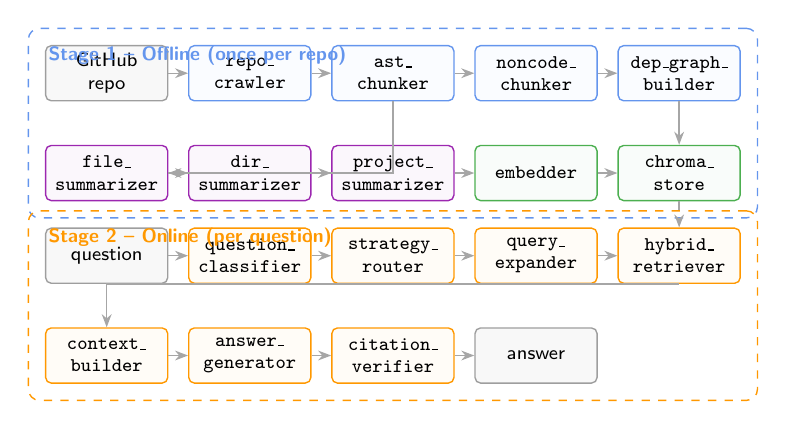
\begin{tikzpicture}[
    font=\sffamily\scriptsize,
    node distance=0.25cm and 0.25cm,
    mod/.style={rectangle, rounded corners=2pt, draw, align=center,
                minimum height=0.7cm, minimum width=1.55cm, line width=0.5pt,
                font=\sffamily\scriptsize\ttfamily, inner sep=2pt},
    iomod/.style={mod, fill=boxgray!40, draw=bordergray, font=\sffamily\scriptsize},
    offmod/.style={mod, fill=boxblue!25, draw=borderblue},
    sumod/.style={mod, fill=boxpurple!30, draw=borderpurple},
    onmod/.style={mod, fill=boxorange!25, draw=borderorange},
    storemod/.style={mod, fill=boxgreen!25, draw=bordergreen},
    arr/.style={-{Stealth[scale=0.9]}, draw=gray!70, line width=0.5pt},
    stage/.style={draw, dashed, inner sep=6pt, rounded corners=4pt, line width=0.5pt},
    stagelabel/.style={font=\sffamily\bfseries\scriptsize}
]

% =========== OFFLINE: ingestion row + summarization/embedding row ===========
\node[iomod]                              (repo)   {GitHub\\repo};
\node[offmod, right=of repo]              (crawl)  {repo\_\\crawler};
\node[offmod, right=of crawl]             (ast)    {ast\_\\chunker};
\node[offmod, right=of ast]               (nonc)   {noncode\_\\chunker};
\node[offmod, right=of nonc]              (dep)    {dep\_graph\_\\builder};

\node[sumod,    below=0.55cm of repo]     (fsum)   {file\_\\summarizer};
\node[sumod,    right=of fsum]            (dsum)   {dir\_\\summarizer};
\node[sumod,    right=of dsum]            (psum)   {project\_\\summarizer};
\node[storemod, right=of psum]            (emb)    {embedder};
\node[storemod, right=of emb]             (chroma) {chroma\_\\store};

\draw[arr] (repo)  -- (crawl);
\draw[arr] (crawl) -- (ast);
\draw[arr] (ast)   -- (nonc);
\draw[arr] (nonc)  -- (dep);
\draw[arr] (ast.south)  |- (fsum.east);
\draw[arr] (fsum)  -- (dsum);
\draw[arr] (dsum)  -- (psum);
\draw[arr] (psum)  -- (emb);
\draw[arr] (emb)   -- (chroma);
\draw[arr] (dep.south) -| (chroma.north);

\node[stage, borderblue, fit=(repo)(dep)(fsum)(chroma)] (stageA) {};
\node[stagelabel, text=borderblue, anchor=north west]
    at ([xshift=4pt, yshift=-3pt]stageA.north west)
    {Stage~1 -- Offline (once per repo)};

% =========== ONLINE: classify row + retrieve/generate row ===========
\node[iomod, below=1.6cm of repo]         (q)      {question};
\node[onmod, right=of q]                  (qcls)   {question\_\\classifier};
\node[onmod, right=of qcls]               (router) {strategy\_\\router};
\node[onmod, right=of router]             (qexp)   {query\_\\expander};
\node[onmod, right=of qexp]               (hybrid) {hybrid\_\\retriever};

\node[onmod, below=0.55cm of q]           (ctx)    {context\_\\builder};
\node[onmod, right=of ctx]                (gen)    {answer\_\\generator};
\node[onmod, right=of gen]                (cite)   {citation\_\\verifier};
\node[iomod, right=of cite]               (ans)    {answer};

\draw[arr] (q)      -- (qcls);
\draw[arr] (qcls)   -- (router);
\draw[arr] (router) -- (qexp);
\draw[arr] (qexp)   -- (hybrid);
\draw[arr] (hybrid.south) -| (ctx.north);
\draw[arr] (ctx)    -- (gen);
\draw[arr] (gen)    -- (cite);
\draw[arr] (cite)   -- (ans);

% offline -> online: index consumed by retriever
\draw[arr, dashed] (chroma.south) to[out=-90, in=90, looseness=0.6] (hybrid.north);

\node[stage, borderorange, fit=(q)(ans)(hybrid)(ctx)] (stageB) {};
\node[stagelabel, text=borderorange, anchor=north west]
    at ([xshift=4pt, yshift=-3pt]stageB.north west)
    {Stage~2 -- Online (per question)};

\end{tikzpicture}
\caption{Concrete module-level pipeline as implemented in \texttt{repoqa/}. Solid arrows show data flow within a stage; the dashed arrow indicates that the online retriever consumes the index produced offline. Stage~1: \texttt{ingestion/}, \texttt{summarization/}, \texttt{embedding/}. Stage~2: \texttt{retrieval/}, \texttt{qa/}.}
\label{fig:pipeline}
\end{figure*}

\subsection{Repository Ingestion \& Hierarchical Summarization}
\label{sec:ingestion}

Given a GitHub repository $R$, we first clone it and traverse its file tree, filtering by language extensions and excluding generated artifacts (e.g., \texttt{node\_modules}, \texttt{build/}).

\paragraph{Code Parsing.}  Use Tree-sitter to parse each source file into an Abstract Syntax Tree (AST) and extract semantic units: functions, classes, module-level code, docstrings, and comments. Following \citet{cast2025}, we employ AST-aware chunking rather than fixed-size sliding windows, ensuring each chunk respects syntactic boundaries.

\paragraph{Non-Code Indexing.}  Create index of non-code files critical for architecture and deployment questions: \texttt{README.md}, \texttt{Dockerfile}, CI/CD configurations, \texttt{package.json}, and environment files. These are chunked using standard text splitting.

\paragraph{Hierarchical Summarization.} Inspired by \citet{tufek2025hierarchical} -- generate summaries at three levels using an LLM:
\begin{itemize}
    \item \textbf{Project-level:} A 1--2 paragraph summary of the repository's purpose, architecture, and key modules, generated from the README and top-level directory listing.
    \item \textbf{Directory-level:} For each top-level directory, a summary describing its role, key files, and relationship to other directories.
    \item \textbf{File-level:} For each source file, a summary of its exports (classes, functions), dependencies, and purpose.
\end{itemize}

\paragraph{Embedding \& Storage.} All chunks (code, non-code, and summaries at each level) are embedded using \texttt{all-mpnet-base-v2} and stored in ChromaDB with metadata (file path, chunk type, directory, language, summary level).

\paragraph{Dependency Graph.} Construct an import graph $G = (V, E)$ where nodes $V$ represent source files and edges $E$ represent import relationships. This enables structural retrieval: if file $A$ is relevant and imports file $B$, then $B$ is likely also relevant.

\subsection{Hybrid Retrieval with Question-Type Routing}
\label{sec:retrieval}

\paragraph{Question Classification.} Classify each developer question into one of three categories using a lightweight LLM prompt:
\begin{itemize}
    \item \textbf{Architecture}: Questions about project structure, module relationships, design patterns (e.g., ``How does authentication work?'').
    \item \textbf{Logic}: Questions about specific function behavior, algorithms, or data transformations (e.g., ``What does \texttt{validate\_token()} do?'').
    \item \textbf{Deployment}: Questions about configuration, build process, environment setup (e.g., ``How is Docker configured?'').
\end{itemize}

\paragraph{Retrieval Strategy Routing.} Each question type triggers a different retrieval strategy:
\begin{itemize}
    \item Architecture $\rightarrow$ Start with project and directory summaries, then expand to file-level chunks in identified modules (top-down).
    \item Logic $\rightarrow$ Start with function-level chunks via semantic search, then include caller/callee context from the dependency graph.
    \item Deployment $\rightarrow$ Prioritize non-code files (Dockerfiles, CI/CD, configs), supplemented by relevant code handlers.
\end{itemize}

\paragraph{Hybrid Fusion.} Within each strategy, proposed to combine three retrieval signals:
\begin{enumerate}
    \item \textbf{Semantic search:} Cosine similarity over embedded chunks (top-$k$=15).
    \item \textbf{BM25:} Keyword matching over raw code text, essential for exact identifier names.
    \item \textbf{Structural search:} Dependency graph traversal---if chunk from file $A$ is retrieved and $A$ imports $B$, boost $B$'s chunks.
\end{enumerate}

Results are fused using Reciprocal Rank Fusion (RRF):
\begin{equation}
    \text{RRF}(d) = \sum_{r \in \{S, B, G\}} \frac{1}{k + \text{rank}_r(d)}
\end{equation}
where $S$, $B$, $G$ denote semantic, BM25, and graph-based rankings respectively, and $k=60$ is a smoothing constant.

\paragraph{Query Expansion.} Before retrieval, we use the LLM to expand the developer's question into additional search terms. For example, ``How does auth work?'' expands to include \{\texttt{authentication}, \texttt{login}, \texttt{token}, \texttt{session}, \texttt{middleware}\}.

\subsection{Structured Prompt Generation}
\label{sec:prompts}

Retrieved context is organized into a structured prompt designed for explanation (not code completion):

\begin{enumerate}
    \item \textbf{System instruction:} Role definition (``You are an expert on the \{repo\_name\} codebase. Explain using ONLY the provided context. Cite file paths and line numbers.'').
    \item \textbf{Project summary:} High-level repo description.
    \item \textbf{Directory summaries:} Summaries of relevant modules.
    \item \textbf{Code chunks:} Retrieved code with file path headers
    \item \textbf{Developer question:} The original question.
\end{enumerate}

This top-down ordering mirrors how a human senior developer would explain code: starting with the big picture, then zooming into details.

\subsection{Answer Generation \& Grounding Verification}
\label{sec:generation}

The LLM generates a structured answer with: (a) a brief overview, (b) detailed explanation with code snippets, and (c) file references. Post-generation, a \textit{citation verifier} checks that every cited file path and function name exists in the repository. Invalid citations are flagged or removed, mitigating hallucination.

\subsection{Cost Accounting}
\label{sec:cost}

Because RepoQA is intended to be re-implementable on either local (Ollama) or commercial (OpenAI / Anthropic / Google) backends, we report cost in two phases that are billed differently. All token counts are obtained from the unified \texttt{TokenCounter} singleton, which wraps the Qwen2.5-7B tokenizer and exposes per-call instrumentation at every LLM site (classifier, query expander, three summarizers, answer generator). This guarantees that chunk-level token budgets and prompt-level token budgets use the same vocabulary.

\paragraph{Offline (once per repository).} Two LLM-driven passes run at indexing time: (i) hierarchical summarization (file $\rightarrow$ directory $\rightarrow$ project), billed as chat input \emph{and} output, and (ii) embedding of all chunks and summaries, billed as input only. We define
\begin{align}
\$_{\text{offline}}\;=\;& T_{\text{emb}} \cdot p_{\text{emb}} \nonumber \\
&+ T_{\text{summ}}^{\text{in}}\cdot p_{\text{chat}}^{\text{in}}
+ T_{\text{summ}}^{\text{out}}\cdot p_{\text{chat}}^{\text{out}}.
\end{align}

\paragraph{Online (per question).} Three LLM calls fire at query time: question classification, query expansion, and structured answer generation. With a context budget of 4{,}000 tokens, the average per-question footprint on the \texttt{pallets/flask} development set is $\approx 4{,}300$ input and $\approx 230$ output tokens.

\paragraph{Per-provider cost (April 2026).}
Table~\ref{tab:cost-providers} reports current public pricing for the chat and embedding tiers we evaluate, together with the projected one-time offline cost and per-question online cost on the flask development repository ($\approx 80$ files, $\approx 5{,}000$ chunks, $\approx 110$ summaries; offline footprint $\approx 350{,}000$ embedding tokens, $\approx 280{,}000$ summarization input, $\approx 20{,}000$ summarization output).

\begin{table*}[h]
\centering
\small
\begin{tabular}{lrrrrr}
\toprule
\textbf{Provider} & \textbf{Chat in} & \textbf{Chat out} & \textbf{Emb} & \textbf{Offline} & \textbf{Online} \\
                  & (\$/1M) & (\$/1M) & (\$/1M) & (\$, one-time) & (\$/question) \\
\midrule
OpenAI GPT-4o-mini + emb-3-small        & 0.15 & 0.60  & 0.020 & 0.06 & 0.0008 \\
OpenAI GPT-4o + emb-3-large             & 2.50 & 10.00 & 0.130 & 0.95 & 0.0131 \\
Anthropic Claude Haiku 4.5 + Voyage-3-lite  & 1.00 & 5.00  & 0.020 & 0.39 & 0.0055 \\
Anthropic Claude Sonnet 4.6 + Voyage-3      & 3.00 & 15.00 & 0.060 & 1.16 & 0.0164 \\
Google Gemini 2.5 Flash + emb-004           & 0.30 & 2.50  & 0.025 & 0.14 & 0.0019 \\
Local Qwen 2.5 7B + nomic-embed (Ollama)    & 0    & 0     & 0     & 0    & 0      \\
\bottomrule
\end{tabular}
\caption{Per-provider cost projection for RepoQA on the \texttt{pallets/flask} development set. Anthropic pairs with Voyage AI for embeddings (no first-party text embedder). Offline cost amortizes across all later questions; online cost is paid per question.}
\label{tab:cost-providers}
\end{table*}

\paragraph{Implications for backend choice.} Three observations follow directly from Table~\ref{tab:cost-providers}. (a)~The summarization pass dominates offline cost across every paid backend, because chat input/output is two orders of magnitude more expensive than embeddings; ablating the summarization layer therefore has a disproportionate effect on \emph{cost} relative to its effect on retrieval recall. (b)~Per-question cost is small in absolute terms ($\le$~\$0.02 for the most expensive configuration), so for evaluation budgets of $\le 1{,}000$ questions the offline phase dominates the total spend---a flask-scale offline run on Claude Haiku ($\$0.39$) is amortized after roughly 70 questions. (c)~Local execution via Ollama eliminates monetary cost but shifts it to GPU/RAM time, which we measure separately and do not include here.

% ============================================================
% 4. DATA
% ============================================================
\section{Datasets}

\subsection{Primary Evaluation: CoReQA}
This paper adopts CoReQA \citep{chen2025coreqa} as the primary evaluation benchmark. CoReQA contains 1,563 QA pairs derived from GitHub issues and comments across 176 repositories in four programming languages (Python: 439, Java: 209, Go: 371, TypeScript: 544). Questions include mixed natural language and code snippets, and reference answers are constructed from community-validated issue discussions (requiring $\geq$3 positive reactions). Each QA pair includes 10 BM25-retrieved reference contexts.

\subsection{Secondary Evaluation: SWE-QA}
SWE-QA \citep{peng2025sweqa} provides architectural comprehension questions specifically targeting cross-module understanding. The experiment is it to evaluate RQ2 (question-type routing effectiveness), as its questions specifically require multi-file reasoning.

\subsection{Development Repositories}
For system development and debugging, select 1--3 open-source repositories of moderate size (5K--50K lines) spanning Python and TypeScript, including at least one repository the development team is unfamiliar with.

\subsection{Data Preprocessing}
For each repository, preprocessing involves: (1)~cloning and file-tree filtering (excluding generated files, binary assets, test fixtures exceeding 1000 lines); (2)~AST-based parsing and chunking with Tree-sitter, targeting chunks of 256--512 tokens; (3)~hierarchical summary generation at three levels; (4)~embedding all chunks and summaries; and (5)~constructing the import dependency graph.

% ============================================================
% 5. EVALUATION METRICS
% ============================================================
\section{Evaluation Metrics}

The experiment uses CoReQA's LLM-as-a-judge framework \citep{chen2025coreqa}, which evaluates generated answers across four dimensions on a 1--10 scale:

\begin{itemize}
    \item \textbf{Accuracy (Acc):} Factual correctness compared to the reference answer.
    \item \textbf{Completeness (Cmpt):} Whether all key aspects of the question are addressed.
    \item \textbf{Relevance (Rel):} Whether the answer addresses the core concern.
    \item \textbf{Clarity (Clar):} Logical structure and readability.
\end{itemize}

The paper additionally report \textbf{Pairwise Comparison Evaluation (PCE)} using Elo scoring for inter-system comparison, \textbf{Retrieval Recall@$k$} ($k$=5, 10) to measure retrieval quality independently of generation, and \textbf{Citation Accuracy} (fraction of cited file paths that exist in the repository).

Each LLM-as-a-judge evaluation is executed 3 times and we report mean $\pm$ standard deviation to account for judge variability ($\approx$5.5\% per CoReQA's validation).

% ============================================================
% 6. EXPERIMENT DESIGN
% ============================================================
\section{Experiment Design}

\subsection{Baselines}
\begin{itemize}
    \item \textbf{No Retrieval:} LLM answers using only the question (lower bound).
    \item \textbf{BM25 Only:} LangChain chunking + BM25 retrieval (CoReQA's reported baseline).
    \item \textbf{Semantic Only:} Embedding-based retrieval without BM25 or structural context.
    \item \textbf{Hybrid (no summaries):} Semantic + BM25 + structural, without hierarchical summaries.
    \item \textbf{RepoQA (full):} Complete system with all components.
\end{itemize}

\subsection{Ablation Study (RQ3)}
To isolate each component's contribution, we run the following ablations, each removing one component:

\begin{table*}[h]
\centering
\small
\begin{tabular}{lcccc}
\toprule
\textbf{Configuration} & \textbf{Summaries} & \textbf{Hybrid (BM25 + sem.)} & \textbf{Query expansion} & \textbf{Type routing} \\
\midrule
Full RepoQA & \checkmark & \checkmark & \checkmark & \checkmark \\
$-$ Summaries & & \checkmark & \checkmark & \checkmark \\
$-$ Hybrid (semantic only) & \checkmark & & \checkmark & \checkmark \\
$-$ Query expansion & \checkmark & \checkmark & & \checkmark \\
$-$ Type routing & \checkmark & \checkmark & \checkmark & \\
BM25 baseline & & & & \\
\bottomrule
\end{tabular}
\caption{Ablation configurations for RQ3. Each row toggles a single component to isolate its marginal contribution.}
\label{tab:ablation}
\end{table*}

\subsection{Expected Results}
Based on CoReQA's reported baselines and our preliminary experiments, we anticipate results in the ranges shown in Table~\ref{tab:expected}.

\begin{table*}[h]
\centering
\small
\begin{tabular}{lcccc}
\toprule
\textbf{System} & \textbf{Accuracy} & \textbf{Completeness} & \textbf{Relevance} & \textbf{Clarity} \\
\midrule
No Retrieval & 6.85 & 6.27 & 7.81 & 8.40 \\
BM25 (reported) & 6.91 & 6.34 & 7.86 & 8.42 \\
RepoQA (expected) & \textbf{7.4--7.8} & \textbf{6.8--7.2} & \textbf{8.0--8.3} & \textbf{8.5--8.7} \\
\bottomrule
\end{tabular}
\caption{Expected performance ranges on CoReQA (Qwen-7B as generator). ``Reported'' values from \citet{chen2025coreqa}.}
\label{tab:expected}
\end{table*}

% ============================================================
% 7. DISCUSSION
% ============================================================
\section{Discussion}

\subsection{How Data and Approach Address the RQs}

\textbf{RQ1} is evaluated by comparing the full RepoQA system against the BM25-only baseline on all 1,563 CoReQA pairs. The four-dimensional LLM-as-a-judge evaluation provides nuanced insight: we expect hybrid retrieval to most improve \textit{completeness} (by retrieving context from multiple related files) and \textit{accuracy} (by providing the correct code definitions rather than superficially similar text).

\textbf{RQ2} is evaluated by comparing question-type-routed retrieval against uniform retrieval, with CoReQA's questions manually categorized into architecture/logic/deployment types. The expectation is the largest gains on architecture questions, where the hierarchical strategy (project $\rightarrow$ directory $\rightarrow$ file) provides crucial structural context that a flat retrieval misses.

\textbf{RQ3} is evaluated through the ablation study (Table~\ref{tab:ablation}), quantifying each component's marginal contribution. The hypothesis that hierarchical summaries contribute most to completeness, hybrid fusion contributes most to accuracy, and query expansion contributes most to relevance.

\subsection{Empirical Findings (Pilot)}
\label{sec:findings}

We report results from a 12-question pilot run on \texttt{pallets/flask} (4 architecture / 4 logic / 4 deployment), executed across all six ablation configurations defined in Table~\ref{tab:ablation}. Gold paths were derived by reading each issue and grounding against the current flask source; gold answers were rewritten from the source code rather than taken from issue comments, after we observed that the original CoReQA-style mining rule (top comment with $\geq 3$ reactions) systematically picks workarounds, opinions, links, or triage notes rather than authoritative explanations (0 of 12 issue comments in our sample were adequate gold answers).

\paragraph{Error distribution.} Each (config, question) row was assigned to one of seven mutually exclusive failure buckets in priority order: retrieval miss, empty context, wrong routing, cited wrong path, unverified citation, low judge quality, or clean pass. Table~\ref{tab:error-dist} reports the distribution per ablation.

\begin{table*}[h]
\centering
\small
\begin{tabular}{lcccccc}
\toprule
\textbf{Configuration} & \textbf{Empty context} & \textbf{Wrong routing} & \textbf{Cited wrong path} & \textbf{Unverified citation} & \textbf{Clean pass} & \textbf{Recall@k (kw)} \\
\midrule
\texttt{bm25\_baseline}  & 4 & 3 & 0 & 3 & 2 & 53.9\% \\
\texttt{full\_repoqa}    & 4 & 3 & 1 & 1 & \textbf{3} & 53.8\% \\
\texttt{no\_expansion}   & 3 & 3 & 2 & 0 & 3 & 41.6\% \\
\texttt{no\_routing}     & 4 & 3 & 2 & 0 & 3 & 51.7\% \\
\texttt{no\_summaries}   & 5 & 2 & 2 & 0 & 3 & 50.6\% \\
\texttt{semantic\_only}  & 5 & 2 & 1 & 1 & 3 & 49.9\% \\
\bottomrule
\end{tabular}
\caption{Error distribution per ablation configuration on the 12-question flask pilot. Buckets are mutually exclusive and evaluated in priority order. ``Retrieval miss'' (0--1 across configs) and ``low judge quality'' (0 across configs) are omitted; each row sums to 12.}
\label{tab:error-dist}
\end{table*}

Three observations. (a)~The dominant failure mode in every configuration is \emph{empty\_context} (3--5 of 12)---answers generated without inline citations---which suggests prompt-level enforcement (require citations or refuse) would yield a larger gain than further retrieval tuning. (b)~Architecture questions are the weakest type: 0 of 4 reached \texttt{clean\_pass} on \texttt{full\_repoqa}, with two failing on empty context and one each on wrong routing and cited-wrong-path. (c)~The keyword-overlap recall metric reports \texttt{full\_repoqa} (53.8\%) and \texttt{bm25\_baseline} (53.9\%) as tied, but the chunk-overlap signal disagrees: \texttt{bm25\_baseline} retrieves a gold-path file in 50\% of questions versus 41.7\% for \texttt{full\_repoqa}---an inversion that the keyword metric obscures. The summary and expansion layers improve citation accuracy (91.7\% vs 75\%) and judge accuracy (6.97 vs 6.69) but at a cost to retrieval precision on this slice.

\paragraph{Systemic finding: citation-path drift.} Across the full 138-row run, 10 of 122 file-path citations (8.2\%) drop the \texttt{src/} prefix---e.g., the model writes \texttt{[flask/app.py]} rather than \texttt{[src/flask/app.py]}. The chunker stores paths as \texttt{src/flask/...} (relative to repo root); the LLM defaults to the human convention of \texttt{flask/...}. Every bare-prefix citation fails the path-equality check in the citation verifier even when the cited claim is correct. This is a structural mismatch between two pipeline components, not a model failure: the trigger condition is decidable (\texttt{path.startswith("flask/")}), the rate is constant across configurations (it does not change when retrieval is ablated, confirming the issue is upstream of retrieval), and a one-line fix in either the verifier (suffix-match instead of equality) or the prompt template (use \texttt{[src/flask/...]} in the example citation) eliminates the entire failure category. We classify this as the only systemic error in our pilot; the remaining failures are model-quality issues without a single closed-form fix.

\paragraph{Summary-level validation.} A separate analysis pass verified all 213 hierarchical summaries (1 project, 31 directory, 181 file) against four deterministic checks (self-mention, length band, scope appropriateness, identifier grounding). Pass rates were 100\%, 90.3\%, and 65.7\% respectively. A 12-summary stratified sample was then hand-reviewed semantically by re-reading the source chunks. The most consequential finding was a \emph{deterministic-pass / semantic-partial} case: the project-level summary passed every automated check but materially omits \texttt{src/flask/} (the actual flask package, 210 indexed chunks) and \texttt{examples/} (90 chunks) from its directory enumeration. Because the project summary gates retrieval for every architecture question, this single defect is a plausible upstream contributor to the architecture-class weakness observed in Table~\ref{tab:error-dist}.

\subsection{Broader Implications}

If the hybrid retrieval approach demonstrates significant improvement over BM25, this has immediate practical implications for AI coding assistants. The same pipeline could be integrated into IDE chat interfaces (Cursor, JetBrains AI), documentation generators, and developer onboarding tools. The hierarchical summarization layer is also independently valuable: it produces human-readable project documentation as a byproduct of the indexing process. The pilot results in Section~\ref{sec:findings} also suggest that any system claiming improvement over BM25 should report chunk-overlap retrieval recall in addition to keyword-overlap recall---the metric inversion we observed indicates that keyword overlap can mask genuine retrieval-quality differences between configurations.

% ============================================================
% 8. CONCLUSION
% ============================================================
\section{Conclusion}

\subsection{Implementation Summary}
\begin{itemize}
    \item Literature review and system architecture for the four-layer pipeline.
    \item \textbf{Stage 1 (offline)}: repository crawler with binary/extension filtering; AST-aware chunker over 8 tree-sitter grammars; non-code chunker for Markdown / TOML / YAML / Dockerfile; import dependency-graph builder; hierarchical summarizer (file $\rightarrow$ directory $\rightarrow$ project) using Qwen2.5-7B via Ollama.
    \item \textbf{Stage 2 (online)}: regex-based and LLM-based question classifiers; per-type strategy router; LLM query expander; BM25 retriever; semantic retriever over ChromaDB (cosine); RRF fusion.
    \item \textbf{Stage 3 (online)}: token-budgeted context builder; type-specific prompt templates; structured ANSWER/CITATIONS/CONFIDENCE answer generator; citation verifier (path + line-range overlap).
    \item \textbf{Stage 4}: Streamlit chat UI with clickable source references.
    \item \textbf{Evaluation infrastructure}: deterministic metrics (recall@k, citation accuracy); LLM-as-a-judge with cross-family pairing (Gemini 2.5 Flash judging Qwen output) and runs-$N$ averaging; ablation runner across six configurations; markdown report generator from JSONL.
    \item \textbf{Dataset construction}: CoReQA-style mining harness for 18 repositories (976 QA pairs), with a curated 23-question \texttt{flask} subset (\texttt{flask\_curated.json}) used for the development pilot. A 12-question gold subset (\texttt{flask\_gold12.json}) was hand-curated with code-grounded answers after we identified that the issue-comment mining rule (top comment by reactions) systematically picks workarounds, opinions, and triage notes rather than authoritative explanations (Section~\ref{sec:findings}).
    \item \textbf{Cost accounting}: unified \texttt{TokenCounter} singleton wrapping the Qwen tokenizer, instrumenting every LLM call site with input/output token logging; offline (summarization + embedding) and online (per-question) cost projections across five paid backends and the local Ollama path (Section~\ref{sec:cost}).
    \item \textbf{Pilot run}: 12 questions $\times$ 6 ablation configurations against the 23-question flask suite, yielding the error distribution in Table~\ref{tab:error-dist}, the metric-inversion finding (BM25 retrieves gold paths in 50\% of questions versus 41.7\% for full RepoQA), and the systemic citation-prefix-drift defect documented in Section~\ref{sec:findings}.
    \item \textbf{Summary validation}: deterministic + qualitative pipeline validating all 213 generated summaries, surfacing one deterministic-pass / semantic-partial case (the project-level summary omits \texttt{src/flask/} and \texttt{examples/}) that plausibly contributes to architecture-class weakness.
\end{itemize}

\subsection{Future Work}
\begin{itemize}
    \item \textbf{Scale beyond $N=12$.} The pilot's bucket-level intervals are too wide for any cell in Table~\ref{tab:error-dist} to be statistically conclusive. Target $N \geq 50$ on the curated flask set, then full CoReQA (1{,}563 pairs across 176 repositories), pending API budget.
    \item \textbf{Wire the dependency graph into retrieval.} The graph is currently constructed at ingestion but not consumed; \texttt{hybrid\_retriever} fuses semantic + BM25 only. Adding a third RRF input ranked by import/call-edge proximity would let us test the original three-way fusion hypothesis.
    \item \textbf{Fix the systemic citation-prefix drift.} A one-line change in either the citation verifier (suffix-match) or the prompt template (use \texttt{[src/flask/...]} in the example) will eliminate the bare-prefix failure category and unbias inter-config comparisons of citation accuracy.
    \item \textbf{Address empty-context failures.} The dominant failure mode (3--5 of 12 per config) is answers without inline citations. A prompt-level constraint that requires citations or explicit refusal would set a floor; an empty-retrieval short-circuit in the QA pipeline would prevent parametric-memory answers when retrieval returns nothing.
    \item \textbf{Drift-resistant gold via PR linkage.} For issues with linked closing PRs, the diff's \texttt{files\_changed} list yields gold paths automatically and is naturally drift-proof at the resolving commit SHA (the SWE-bench mechanism). Estimated coverage on flask: 60--70\%.
    \item \textbf{Symbol-anchored chunk identity.} Chunk IDs currently hash \texttt{(repo\_path, start\_line)}, which breaks under refactor. Re-keying on \texttt{(repo\_path, symbol\_name, symbol\_kind)} eliminates drift from line-shifting refactors and aligns with how Sourcegraph SCIP and Cursor track references.
    \item \textbf{Improve the project-level summary.} The current summary's omission of \texttt{src/flask/} and \texttt{examples/} should be addressed by making the project summarizer enumerate top-level directories from the index rather than from the file-summary aggregation, which evidently dropped two of them.
    \item \textbf{Layered summary verification.} Pair the deterministic checks (already deployed) with an LLM-as-judge faithfulness pass on (a)~all project summaries and (b)~all top-level directory summaries, since these have the largest blast radius. Mutation-tested calibration of the judge is the path to scaling this without proportional human work.
\end{itemize}

\subsection{Limitations and Mitigations}
\begin{itemize}
    \item \textbf{Statistical power.} At $N=12$, individual bucket counts in Table~\ref{tab:error-dist} have wide intervals; conclusions are directional. Mitigation: report effect sizes alongside counts and treat $N=12$ findings as hypothesis-generating until the larger run completes.
    \item \textbf{Self-evaluation bias in LLM-as-judge.} The Qwen generator and the Gemini judge are different model families by design; for the 12-question pilot the judge accuracies cluster at 6.6--7.0, lower than typical generator-side self-grading.
    \item \textbf{Gold-label correctness.} The 12-question gold subset was hand-curated by reading the flask source directly; entries are flagged for human verification but every gold path was confirmed to exist in the indexed corpus before commit.
    \item \textbf{LLM API cost drift.} \texttt{TokenCounter}-instrumented per-call logging plus the offline/online cost projection table (Table~\ref{tab:cost-providers}) bound spending in advance and let configuration changes be screened for cost impact before commit.
    \item \textbf{Evaluation variance.} The judge is run $N=3$ times per (config, question) and we report mean $\pm$ std on each cell; deterministic metrics carry no variance.
\end{itemize}

% ============================================================
% REFERENCES
% ============================================================
\bibliography{references}    % Points to your references.bib file

\end{document}
